\subsubsection{bringit::client::chat::ChatSource}

\label{bringit::client::chat::ChatSource}
\begin{figure}[H]
	\centering
	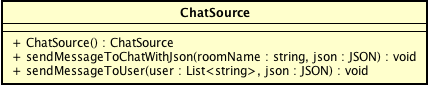
\includegraphics[scale=0.5]{Sezioni/SottosezioniST/img/app/ChatSource.png}
	\caption{bringit::client::chat::ChatSource}
\end{figure}

\begin{itemize}
\item \textbf{Descrizione}: Interfaccia di comunicazione con la chat Rocket.Chat.
\item \textbf{Utilizzo}: La classe viene utilizzata per l'invio di messaggi nei vari canali di chat di Rocket.Chat.
\item \textbf{Attributi}: 
\item \textbf{Metodi}:
	\begin{itemize}
	\item \textit{public ChatSource():ChatSource}\\
	Il costruttore della classe ChatSource.
	\item \textit{public sendMessageToChatWithJson(roomName:string,json:JSONObject):void}\\
	Questo metodo invia un messaggio direttamente a un canale di Rocket.Chat.
			\\ \textbf{Parametri}: \begin{itemize}
				\item \textit{roomName:string}\\
				Il nome (unico) della chat alla quale si vuole mandare il messaggio.
				\item \textit{json:JSONObject}\\
				Il messaggio che si vuole mandare, rappresentato con un oggetto di tipo json.
			\end{itemize}
	\item \textit{public sendMessageToUser(user:string[],json:JSONObject):void}\\
	Questo metodo invia un messaggio direttamente a utente di Rocket.Chat.
			\\ \textbf{Parametri}: \begin{itemize}
				\item \textit{user:string[]}\\
				Array contenente tutti gli utenti ai quali si vuole mandare il messaggio
				\item \textit{json:JSONObject}\\
				Il messaggio che si vuole mandare, rappresentato con un oggetto di tipo json.
			\end{itemize}
	\end{itemize}
\end{itemize} 

